\subsection{Why Filtering ?}
\begin{frame}
	\frametitle\insertsection
	\framesubtitle\empty
	\begin{center}
		\Large \textbf{\insertsubsection}
	\end{center}
\end{frame}
\begin{frame}
	\frametitle\insertsection
	\framesubtitle\insertsubsection
	\vspace{-2em}
	\begin{itemize}
		\item {Reduce errors in measured position through weighted averaging.}
		\item {Estimate target velocity and sometimes target acceleration.}
		\item {Better prediction of future target position for specific purposes.}
	\end{itemize}
\end{frame}
\subsection{Models \& Problems}
\begin{frame}
	\frametitle\insertsection
	\framesubtitle\empty
	\begin{center}
		\Large \textbf{\insertsubsection}
	\end{center}
\end{frame}
\begin{frame}
	\frametitle\insertsection
	\framesubtitle\insertsubsection
	\vspace{-1.5em}
	\begin{block}{State Equation}
		\begin{itemize}
			\item {A mathematical model of how the state $\mathbf{X}_{k}$ varies in time; so-called Process Model or Motion Model:}
			\begin{align*}
				\mathbf{X}_k= \mathbf{F}(\mathbf{X}_{k-1})+u_k
			\end{align*}
			\item {$\mathbf{X}_k$: the track state vector}
			\item {$\mathbf{F}$: the state transition matrix or equation of motion}
			\item {$u_k$: the white gaussian dynamic or process noise independent from the initial state $\mathbf{X}_0$ so that:}
			\begin{align*}
				E[u_{k}u^\intercal_{j}] = \mathbf{Q}_k\delta_{kj} = 
				\begin{cases}
					0 & \text{if $k \neq j$} \\
					v^u_k & \text{otherwise}
				\end{cases}
			\end{align*}
		\end{itemize}
	\end{block}
\end{frame}
\begin{frame}
	\frametitle\insertsection
	\framesubtitle\insertsubsection
	\vspace{-1.5em}
	\begin{block}{Observation Equation}
		\begin{itemize}
			\item {The equation are related to the unknown state vector to predicted observations or measurements:}
			\begin{align*}
				\mathbf{Z}_k= \mathbf{H}(\mathbf{X}_k)+w_k
			\end{align*}
			\item {$\mathbf{X}_k$: the measurement vector}
			\item {$\mathbf{H}$: the observation matrix}
			\item {$w_k$: the white gaussian measurement noise independent from the initial state $x_0$ so that:}
			\begin{align*}
				E[w_{k}w^\intercal_{j}] = \mathbf{R}_k\delta_{kj} = 
				\begin{cases}
					0 & \text{if $k \neq j$} \\
					v^w_k & \text{otherwise}
				\end{cases}
			\end{align*}
		\end{itemize}
	\end{block}
\end{frame}
\begin{frame}
	\frametitle\insertsection
	\framesubtitle\insertsubsection
	\begin{block}{Problems}
		The estimation problem of state $\mathbf{X}_k$ of the system from measurements $z_k$ can be divided in 3 distinct problems according to measurement interval:\\
		\begin{itemize}
			\item {\textbf{Correction:} Estimation of $\mathbf{X}_k$ from ${[\mathbf{Z}_1,...,\mathbf{Z}_N]}$ with $k=N$}
			\item {\textbf{Prediction:} Estimation of $\mathbf{X}_k$ from ${[\mathbf{Z}_1,...,\mathbf{Z}_N]}$ with $k>N$}
			\item {\textbf{Smoothing:} Estimation of $\mathbf{X}_k$ from ${[\mathbf{Z}_1,...,\mathbf{Z}_N]}$ with $k<N$}
		\end{itemize}
	\end{block}
\end{frame}
\begin{frame}
	\frametitle\insertsection
	\framesubtitle\insertsubsection
	\begin{block}{Measurement Model : Examples}
		\begin{itemize}
			\item {Simple cartesian}
			\begin{align*}
				\mathbf{Z}_{k} =[x_{k} \ y_{k} ]^\intercal + e_{k}
			\end{align*}
			\item {Range}
			\begin{align*}
				\mathbf{Z}_{k} =\sqrt{x^2_k + y^2_k} + e_k
			\end{align*}
			\item {Bearing only}
			\begin{align*}
				\mathbf{Z}_{k} = \textup{atan2}(y_k,x_k)+ e_k
			\end{align*}
		\end{itemize}
	\end{block}
\end{frame}
\begin{frame}
	\frametitle\insertsection
	\framesubtitle\insertsubsection
	\begin{block}{Motion Models} \footnotesize
		\textbf{Constant Velocity (CV) Model :}
		\begin{align*}
			\mathbf{X}_k\triangleq
			\begin{bmatrix}
				x_k\\\dot{x}_k
			\end{bmatrix} =
			\begin{bmatrix}
				1&T\\0&1
			\end{bmatrix}  
			\begin{bmatrix}
				x_{k-1}\\\dot{x}_{k-1}
			\end{bmatrix} + 
			\begin{bmatrix}
				{T^{2}}/2\\T
			\end{bmatrix} a_k
		\end{align*}
		where $a_{k} \sim N(0, \sigma^{2}_{a})$ is a white noise.\\
		\vspace{1em}
		\textbf{Constant Acceleration (CA) Model :}
		\begin{align*}
			\mathbf{X}_k\triangleq
			\begin{bmatrix}
				x_k\\\dot{x}_k\\\ddot{x}_k
			\end{bmatrix} = 
			\begin{bmatrix}
				1&T&{T^2}/2 \\ 0&1&T \\ 0&0&1
			\end{bmatrix}
			\begin{bmatrix}
				x_{k-1}\\\dot{x}_{k-1}\\\ddot{x}_{k-1}
			\end{bmatrix} + 
			\begin{bmatrix}
				{T^{2}}/{2} \\ T \\ 1
			\end{bmatrix}  \eta_{k}
		\end{align*}
		where $\eta _{k} \sim N(0, \sigma ^{2}_{ \eta })$ is a white noise.
	\end{block}
\end{frame}
\begin{frame}
	\frametitle\insertsection
	\framesubtitle\insertsubsection
	\vspace{-1em}
	\begin{block}{Motion Models (cont'd)}
		\footnotesize
		\textbf{Coordinated Turn (CT) Model :}
		\begin{align*}
			\mathbf{X}_{k} &\triangleq
			\begin{bmatrix}
				x_k & y_k & \dot{x}_k & \dot{y}_k & \omega_k
			\end{bmatrix}^\intercal \\
			\mathbf{X}_k &=
			\begin{bmatrix}
				1 & 0 &\cfrac{\sin(\omega_{k-1}T)}{\omega_{k-1}} & -\cfrac{1-\cos(\omega_{k-1}T) }{\omega_{k-1})} & 0 \\
				0 & 1 & \cfrac{1- \cos(\omega _{k-1}T) }{\omega_{k-1}} & \cfrac{\sin(\omega_{k-1}T) }{\omega_{k-1}} & 0 \\
				0 & 0 & \cos(\omega_{k-1}T) & -\sin(\omega_{k-1}T) & 0 \\
				0 & 0 & \sin(\omega_{k-1}T) & \cos(\omega_{k-1}T) & 0 \\
				0 & 0 & 0 & 0 & 1
			\end{bmatrix} \mathbf{X}_{k-1}
			+
			\begin{bmatrix}
				{T^{2}}/2 & 0 & 0 \\
				0 & {T^{2}}/2 & 0 \\
				T & 0 & 0 \\
				0 & T & 0 \\
				0 & 0 & 1
			\end{bmatrix} \eta _{k}
		\end{align*}
	\end{block}
\end{frame}
\subsection{Kalman Filtering}
\begin{frame}
	\frametitle\insertsection
	\framesubtitle\empty
	\begin{center}
		\Large \textbf{\insertsubsection}
	\end{center}
\end{frame}
\begin{frame}
	\frametitle\insertsection
	\framesubtitle\insertsubsection
	\begin{block} {Kalman Filter}
		\begin{itemize}
			\item {Introduced by Kalman (1960), has been one of most widely used estimation algorithms.}
			\item {A recursive and statistically estimator}
			\item {The optimal minimum mean square error (MMSE) estimation for linear, gaussian systems.}
		\end{itemize}
	\end{block}
\end{frame}
%\begin{frame}
%	\frametitle\insertsection
%	\framesubtitle\insertsubsection
%	\begin{block}{Process Noise}
%		\begin{itemize}
%			\item {Process noise $\mathbf{Q}_k$ is how a target deviate its position from assumed motion model.}
%			\item {Example of CV white noise model:}
%			\begin{align*}
%				\mathbf{Q}_k = \sigma^2_a
%				\begin{bmatrix}
%					\dfrac{\Delta t^4}{4} & \dfrac{\Delta t^3}{2} \\
%					\dfrac{\Delta t^3}{2} & \Delta t^2 \\
%				\end{bmatrix}
%			\end{align*}
%		\end{itemize}
%	\end{block}
%\end{frame}
\begin{frame}
	\frametitle\insertsection
	\framesubtitle\insertsubsection
	\vspace{-1.5em}
	\begin{block} {Kalman Filtering Parameters}
		\begin{table}\small
			\begin{tabular}{p{4cm}c}
				Predicted State Estimate: & $\hat{\mathbf{X}}_{k|k-1}= \mathbf{F}_{k|k-1} \hat{\mathbf{X}}_{k-1|k-1}$ \\ \\
				Predicted Covariance: & $\mathbf{P}_{k|k-1}= \mathbf{F}_{k|k-1} \mathbf{P}_{k-1|k-1} \mathbf{F}^\intercal_{k|k-1} + \mathbf{Q}_{k|k-1}$ \\ \\
				Residual (Innovation): & $\mathbf{\nu}_k = \mathbf{Z}_k - \hat{\mathbf{Z}}_{k|k-1} = \mathbf{Z}_k - \mathbf{H} \hat{\mathbf{X}}_{k|k-1}$ \\ \\
				Residual Covariance: & $\mathbf{S}_k = \mathbf{HP}_{k|k-1}\mathbf{H}^\intercal - \mathbf{R}_k$ \\ \\
				Kalman Gain: & $\mathbf{K}_k = \mathbf{P}_{k|k-1} \mathbf{H}^\intercal \mathbf{S}^{-1}_k$ \\ \\
				Track State Estimate: & $\hat{\mathbf{X}}_{k|k} = \hat{\mathbf{X}}_{k|k-1} + \mathbf{K}_k \mathbf{\nu}_k$ \\ \\
				Covariance: & $\mathbf{P}_{k|k} = (\mathbf{I} - \mathbf{K}_k \mathbf{H}) \mathbf{P}_{k|k-1} (\mathbf{I} - \mathbf{K}_k \mathbf{H})^\intercal + \mathbf{K}_k\mathbf{R}_k\mathbf{K}^\intercal_k$
			\end{tabular}
		\end{table}
	\end{block}
\end{frame}
%\begin{frame}
%	\frametitle\insertsection
%	\framesubtitle\insertsubsection
%	\begin{block}{Track State Prediction}
%		\begin{itemize}
%			\item {Using the state vector and state transition matrix, the equation for predicting the state can be written as:}
%			\begin{align*}
%				\hat{\mathbf{X}}_{k|k-1}= \mathbf{F}_{k|k-1} \hat{\mathbf{X}}_{k-1|k-1}
%			\end{align*}
%		\end{itemize}
%	\end{block}
%\end{frame}
%\begin{frame}
%	\frametitle\insertsection
%	\framesubtitle\insertsubsection
%	\vspace{-1em}
%	\begin{block}{Track Covariance Matrix}
%		\begin{itemize}
%			\item {A matrix $\mathbf{P}_k$ containing all of the variance quantities related to all elements of the state.}
%			\item {The diagonal elements are the variances of the members of the state vector.}
%			\item {The off-diagonal elements are the covariance between any two state vector members.}
%			\begin{align*}
%				\mathbf{P}_k =
%				\begin{bmatrix}
%					{\sigma_x}^2 & \sigma_{xy} & \sigma_{xz} \\
%					\sigma_{yx} & {\sigma_y}^2 & \sigma_{yz} \\
%					\sigma_{zx} & \sigma_{zy} & {\sigma_z}^2 \\
%				\end{bmatrix}
%			\end{align*}
%		\end{itemize}
%	\end{block}
%\end{frame}
%\begin{frame}
%	\frametitle\insertsection
%	\framesubtitle\insertsubsection
%	\begin{block}{Track Covariance Prediction}
%		\begin{itemize}
%			\item {The covariance matrix is predicted using state transition matrix.}
%			\item {Process noise is included in the prediction of the covariance matrix.}
%			\item {Process noise is included in the prediction of the covariance matrix.}
%			\begin{align*}
%				\mathbf{P}_{k|k-1}= \mathbf{F}_{k|k-1} \mathbf{P}_{k-1|k-1} \mathbf{F}^\intercal_{k|k-1} + \mathbf{Q}_{k|k-1}
%			\end{align*}
%		\end{itemize}
%	\end{block}
%\end{frame}
%\begin{frame}
%	\frametitle\insertsection
%	\framesubtitle\insertsubsection
%	\vspace{-1em}
%	\begin{block}{Measurement Vector}
%		\begin{itemize}
%			\item {The vector $\mathbf{Z}_k$ is a column vector containing the new measurement from an example:}
%			\begin{align*}
%				\mathbf{Z}_k =
%				\begin{bmatrix}
%					x_k & y_k & z_k
%				\end{bmatrix}^\intercal
%			\end{align*}
%		\end{itemize}
%	\end{block}
%	\begin{block}{Measurement Covariance Matrix}
%		\begin{itemize}
%			\item {The matrix $\mathbf{R}_k$ contains the variances of measured quantities and covariances if required.}
%			\begin{align*}
%				\mathbf{R}_k =
%				\begin{bmatrix}
%					\sigma^2_x & 0 & 0 \\
%					0 & \sigma^2_y & 0 \\
%					0 & 0 & \sigma^2_z
%				\end{bmatrix}
%			\end{align*}
%		\end{itemize}
%	\end{block}
%\end{frame}
%\begin{frame}
%	\frametitle\insertsection
%	\framesubtitle\insertsubsection
%	\vspace{-1em}
%	\begin{block}{Observation Matrix}
%		\begin{itemize}
%			\item {The state vector and the covariance matrix include all of the state quantities.}
%			\item {The observation matrix $\mathbf{H}$ enables the parts of these related to the measures quantities to be extracted from all elements.}
%		\end{itemize}
%	\end{block}
%	\begin{block}{Predicted Measurement Vector}
%		\begin{itemize}
%			\item {With the observation matrix $\mathbf{H}$ and the predicted state vector $\mathbf{X}_{k|k-1}$, predicted measurement vector $\mathbf{Z}_k$ can be determined:}
%			\begin{align*}
%				\hat{\mathbf{Z}}_{k|k-1} = \mathbf{H} \hat{\mathbf{X}}_{k|k-1}
%			\end{align*}
%		\end{itemize}
%	\end{block}
%\end{frame}
%\begin{frame}
%	\frametitle\insertsection
%	\framesubtitle\insertsubsection
%	\vspace{-1em}
%	\begin{block}{Residual (Innovation) Vector}
%		\begin{itemize}
%			\item {The residual $\mathbf{\nu}_k$ is the difference between the measurement and the predicted measurement:}
%			\begin{align*}
%				\mathbf{\nu}_k = \mathbf{Z}_k - \hat{\mathbf{Z}}_{k|k-1} = \mathbf{Z}_k - \mathbf{H} \hat{\mathbf{X}}_{k|k-1}
%			\end{align*}
%		\end{itemize}
%	\end{block}
%	\begin{block}{Residual (Innovation) Covariance Matrix}
%		\begin{itemize}
%			\item {The covariance matrix $\mathbf{S}_k$ is expressed in terms of the predicted track covariance matrix related to the measured quantities with the measurement covariance matrix:}
%			\begin{align*}
%				\mathbf{S}_k = \mathbf{HP}_{k|k-1}\mathbf{H}^\intercal - \mathbf{R}_k
%			\end{align*}
%		\end{itemize}
%	\end{block}
%\end{frame}
%\begin{frame}
%	\frametitle\insertsection
%	\framesubtitle\insertsubsection
%	\vspace{-1em}
%	\begin{block}{Gain Matrix}
%		\begin{itemize}
%			\item {The gain matrix $\mathbf{K}_k$ determines the relative weight given to the predicted and the new measurement to update the state.}
%			\begin{align*}
%				\mathbf{K}_k = \mathbf{P}_{k|k-1} \mathbf{H}^\intercal \mathbf{S}^{-1}_k
%			\end{align*}
%		\end{itemize}
%	\end{block}
%	\begin{block}{Track State Vector Update}
%		\begin{itemize}
%			\item {The predicted state can then be updated to obtain a new track estimated.}
%			\begin{align*}
%				\hat{\mathbf{X}}_{k|k} = \hat{\mathbf{X}}_{k|k-1} + \mathbf{K}_k \mathbf{\nu}_k
%			\end{align*}
%		\end{itemize}
%	\end{block}
%\end{frame}
%\begin{frame}
%	\frametitle\insertsection
%	\framesubtitle\insertsubsection
%	\vspace{-1em}
%	\begin{block}{Track Covariance Matrix Update}
%		\begin{itemize}
%			\item {The predicted covariance is also updated to updated to obtain the covariance of the new state estimate.}
%			\begin{align*}
%				\mathbf{P}_{k|k} = (\mathbf{I} - \mathbf{K}_k \mathbf{H}) \mathbf{P}_{k|k-1} (\mathbf{I} - \mathbf{K}_k \mathbf{H})^\intercal + \mathbf{K}_k\mathbf{R}_k\mathbf{K}^\intercal_k
%			\end{align*}
%		\end{itemize}
%	\end{block}
%\end{frame}
\begin{frame}
	\frametitle\insertsection
	\framesubtitle\insertsubsection
	\vspace{-2em}
	\begin{figure}
		\caption{\textbf{Kalman Filtering Process}}
		\scalebox{0.667}{\begin{tikzpicture}[xscale=1,yscale=1,
	square/.style={rectangle, minimum height=22mm, draw=black, align=center},
	label/.style={text width=5mm},
	node distance= 3cm and 1cm, >=stealth]
	
	%Nodes
	\node[square]	(apriori)	at (0,0)	{
		\textbf{A priori input:}\\ \\
		$\hat{\mathbf{X}}_{k-1|k-1}=\mathbf{X}_0$\\
		$\mathbf{P}_{k-1|k-1}=\mathbf{P}_0$
	};
	\node[square, minimum height=10mm]	(init)	[right of=apriori]	{
		$k=1$
	};
	\node[square, xshift=2cm]	(prediction)	[right of=init]	{
		\textbf{Prediction:}\\ \\
		$\hat{\mathbf{X}}_{k|k-1}= \mathbf{F}_{k|k-1} \hat{\mathbf{X}}_{k-1|k-1}$\\
		$\mathbf{P}_{k|k-1}= \mathbf{F}_{k|k-1} \mathbf{P}_{k-1|k-1} \mathbf{F}^\intercal_{k|k-1} + \mathbf{Q}_{k|k-1}$
	};

	\node[square, xshift=3cm]	(residual)	[right of=prediction]	{
		\textbf{Residual computation:}\\ \\
		$\mathbf{\nu}_k = \mathbf{Z}_k - \mathbf{H} \hat{\mathbf{X}}_{k|k-1}$\\
		$\mathbf{S}_k = \mathbf{HP}_{k|k-1}\mathbf{H}^\intercal - \mathbf{R}_k$
	};

	\node[square]	(gain)	[below of=residual]	{
		\textbf{Gain computation:}\\ \\
		$\hat{\mathbf{X}}_{k|k} = \hat{\mathbf{X}}_{k|k-1} + \mathbf{K}_k \mathbf{\nu}_k$\\
		$\mathbf{K}_k = \mathbf{P}_{k|k-1} \mathbf{H}^\intercal \mathbf{S}^{-1}_k$
	};

	\node[square]	(filter)	[below of=gain]	{
		\textbf{Filter Update:}\\ \\
		$\hat{\mathbf{X}}_{k|k} = \hat{\mathbf{X}}_{k|k-1} + \mathbf{K}_k \mathbf{\nu}_k$\\
		$\mathbf{P}_{k|k} = (\mathbf{I} - \mathbf{K}_k \mathbf{H}) \mathbf{P}_{k|k-1}$
	};
	\node[square, xshift=-4cm, minimum height=10mm]	(increment)	[left of=filter]	{$k=k+1$};
	
	\node[label, xshift=-1.8cm]	(zk)	[above left of=prediction]	{$\mathbf{Z}_k$};
	
	%Lines
	\draw[black, thick, ->] (apriori) -- (init);
	%\draw[black, thick, ->] (init.20) -- ++(0.9,0);
	\draw[black, thick, ->] (zk) |- (prediction.170);
	\draw[black, thick, ->] (init) -- (prediction);
	\draw[black, thick, ->] (prediction) -- (residual);
	\draw[black, thick, ->] (residual) -- (gain);
	\draw[black, thick, ->] (gain) -- (filter);
	%\draw[black, thick, ->] (filter.170) -| (prediction);
	%\draw[balck, thick, ->]	(filter.190) -- ()
	\draw[black, thick, ->]	(filter) -- (increment);
	\draw[black, thick, ->] (increment) -- ++(-3,0) |- (prediction.190);
\end{tikzpicture}}
	\end{figure}
\end{frame}
\begin{frame}
	\frametitle\insertsection
	\framesubtitle\insertsubsection
	\vspace{-2em}
	\textbf{Step 1 : Prediction}
	\begin{figure}
		\scalebox{1}{\begin{tikzpicture}[xscale=1,yscale=1,
	round/.style={circle, inner sep=0pt, fill=red!50, opacity=0.75, align=center},
	point/.style={circle, inner sep=0pt, minimum size=2mm, align=center},
	oval/.style={ellipse, fill=gray!50, opacity=0.75},
	label/.style={text width=15mm, align=center},
	node distance= 3cm and 1cm, >=stealth]
		
	%Nodes
	\node[oval, minimum height=1.5cm, minimum width=2cm, rotate=60]	(area0)	at	(0,0)	{};
	\node[point, minimum size=1.5mm, fill=black]	(p0)	at	(0,0)	{};
	
	\node[oval, minimum height=2cm, minimum width=2.5cm, rotate=60]	(area1)	at	(2,2)	{};
	\node[point, minimum size=1.5mm, fill=black]	(p1)	at	(2,2)	{};
	
	\node[label]	(l1)	at	(1,-2)	{$\hat{\mathbf{X}}_{k-1|k-1}$};
	\node[label]	(l2)	at	(4,0)	{$\hat{\mathbf{X}}_{k|k-1}$};
	\node[label, font=\scriptsize, text width=20mm]	(l3)	at	(5,3.1)	{True Trajectory};
	
	%Lines
	\draw[black, dashed, -] (p0) -- (p1);
	\draw[black, thick,->] (p0) -- ++(0.5,0.5);
	\draw[black, thick, -] (p0) -- ++(0.75,0.25);
	\draw[black, thick, -] (p0) -- ++(0.25,0.75);
	\draw[black, thick, ->] (p1) -- ++(0.5,0.5);
	\draw[black, thick, -] (p1) -- ++(0.75,0.25);
	\draw[black, thick, -] (p1) -- ++(0.25,0.75);
	
	\draw[black, ->] (l1) -- (0.1,-0.1);
	\draw[black, ->] (l2) -- (2.1, 1.9);
	
	\draw[blue!50, thick, ->] (-2,-1) -- (4, 3);
\end{tikzpicture}}
	\end{figure}
\end{frame}
\begin{frame}
	\frametitle\insertsection
	\framesubtitle\insertsubsection
	\vspace{-1em}
	\textbf{Step 2 : Residual Computation}
	\begin{figure}
		\scalebox{1}{\begin{tikzpicture}[xscale=1,yscale=1,
	round/.style={circle, inner sep=0pt, fill=red!50, opacity=0.75, align=center},
	point/.style={circle, inner sep=0pt, minimum size=2mm, align=center},
	oval/.style={ellipse, fill=gray!50, opacity=0.75},
	label/.style={text width=5mm, align=center},
	node distance= 3cm and 1cm, >=stealth]
		
	%Nodes
	\node[oval, minimum height=1.5cm, minimum width=2cm, rotate=60]	(area0)	at	(0,0)	{};
	\node[point, minimum size=1.5mm, fill=black]	(p0)	at	(0,0)	{};
	
	\node[oval, fill=green!50, opacity=0.5, minimum height=3cm, minimum width=4.5cm, rotate=-80]	(residual)	at	(2,2)	{};
	
	\node[oval, minimum height=2cm, minimum width=2.5cm, rotate=60]	(area1)	at	(2,2)	{};
	\node[point, minimum size=1.5mm, fill=black]	(p1)	at	(2,2)	{};
	
	\node[point, minimum size=1.5mm, fill=blue!80]	(m1)	at	(1.9,3.1)	{};
	
	\node[label]	(l1)	at	(1,-2)	{$\hat{\mathbf{X}}_{k-1|k-1}$};
	\node[label]	(l2)	at	(4,0)	{$\hat{\mathbf{Z}}_{k|k-1}$};
	\node[label, font=\scriptsize, text width=20mm]	(l3)	at	(5,3.1)	{True Trajectory};
	\node[label]	(l4)	at	(5,4)	{$\mathbf{Z}_k$};
	\node[label]	(l5)	at	(-1,3)	{$\mathbf{\nu}_k$};
	
	%Lines
	\draw[black, dashed, -] (p0) -- (p1);
	\draw[black, thick,->] (p0) -- ++(0.5,0.5);
	\draw[black, thick, -] (p0) -- ++(0.75,0.25);
	\draw[black, thick, -] (p0) -- ++(0.25,0.75);
	\draw[black, thick, ->] (p1) -- ++(0.5,0.5);
	\draw[black, thick, -] (p1) -- ++(0.75,0.25);
	\draw[black, thick, -] (p1) -- ++(0.25,0.75);
	
	\draw[black, thick, -] (p1) -- ++(-0.1,1.1);
	
	\draw[black, ->] (l1) -- (0.1,-0.1);
	\draw[black, ->] (l2) -- (2.1, 1.9);
	\draw[black, ->] (l4) -- (m1);
	\draw[black, ->] (l5) -- (1.95,2.55);
	
	\draw[blue!50, thick, ->] (-2,-1) -- (4, 3);
\end{tikzpicture}}
	\end{figure}
\end{frame}
\begin{frame}
	\frametitle\insertsection
	\framesubtitle\insertsubsection
	\textbf{Step 3+4 : Gain Computation \& Filter Update}
	\begin{figure}
		\scalebox{1}{\begin{tikzpicture}[xscale=1,yscale=1,
	round/.style={circle, inner sep=0pt, fill=red!50, opacity=0.75, align=center},
	point/.style={circle, inner sep=0pt, minimum size=2mm, align=center},
	oval/.style={ellipse, fill=gray!50, opacity=0.75},
	label/.style={text width=5mm, align=center},
	node distance= 3cm and 1cm, >=stealth]
		
	%Nodes
	\node[oval, minimum height=1.5cm, minimum width=2cm, rotate=60]	(area0)	at	(0,0)	{};
	\node[point, minimum size=1.5mm, fill=black]	(p0)	at	(0,0)	{};
	
	\node[oval, minimum height=1cm, minimum width=2cm, rotate=92]	(area1)	at	(1.95,2.55)	{};
	\node[point, minimum size=1.5mm, fill=black]	(p1)	at	(2,2)	{};
	
	\node[point, minimum size=1.5mm, fill=blue!80]	(m1)	at	(1.9,3.1)	{};
	
	\node[label]	(l1)	at	(1,-1)	{$\hat{\mathbf{X}}_{k-1|k-1}$};
	\node[label]	(l2)	at	(4,0)	{$\hat{\mathbf{Z}}_{k|k-1}$};
	\node[label, font=\scriptsize, text width=20mm]	(l3)	at	(5,3.1)	{True Trajectory};
	\node[label]	(l4)	at	(5,4)	{$\mathbf{Z}_k$};
	\node[label, text width=10mm]	(l5)	at	(-1,3)	{$\hat{\mathbf{X}}_{k|k}$};
	
	%Lines
	\draw[black, dashed, -] (p0) -- (p1);
	\draw[black, thick,->] (p0) -- ++(0.5,0.5);
	\draw[black, thick, -] (p0) -- ++(0.75,0.25);
	\draw[black, thick, -] (p0) -- ++(0.25,0.75);
	\draw[black, thick, ->] (p1) -- ++(0.5,0.5);
	\draw[black, thick, -] (p1) -- ++(0.75,0.25);
	\draw[black, thick, -] (p1) -- ++(0.25,0.75);
	
	\draw[black, thick, -] (p1) -- ++(-0.1,1.1);
	
	\draw[black, ->] (l1) -- (0.1,-0.1);
	\draw[black, ->] (l2) -- (2.1, 1.9);
	\draw[black, ->] (l4) -- (m1);
	\draw[black, ->] (l5) -- (1.9,2.55);
	
	\draw[blue!50, thick, ->] (-2,-1) -- (4, 3);
	
	\node[point, minimum size=1.5mm, fill=red, draw=black]	(m1)	at	(1.95,2.55)	{};
\end{tikzpicture}}
	\end{figure}
\end{frame}
\begin{frame}
	\frametitle\insertsection
	\framesubtitle\insertsubsection
	\vspace{-2em}
	\begin{figure}
		\caption{\textbf{Evolution of area uncertainties}}
		\scalebox{0.75}{\begin{tikzpicture}[xscale=1,yscale=1,
	oval/.style={ellipse, fill=green!50, opacity=0.75, rotate=45},
	label/.style={text width=15mm, align=center},
	node distance= 3cm and 1cm, >=stealth]
		
	%Nodes
	\node[oval, minimum height=1.5cm, minimum width=3cm]	(area0)	at	(-1,0)	{};
	\node[oval, minimum height=2cm, minimum width=4cm]	(area1)	at (4,0)	{};
	\node[oval, minimum height=1cm, minimum width=2cm]	(area2)	at (4,-3)	{};
	\node[oval, minimum height=1.25cm, minimum width=2.5cm]	(area3)	at (7.5,-3)	{};
	\node[oval, minimum height=0.7cm, minimum width=1.4cm]	(area4)	at (7.5,-5.5)	{};
	%\node[label, font=\scriptsize, text width=20mm]	(l3)	at	(5,3.1)	{True Trajectory};
	
	%Lines
	\draw[black, thick, ->] (area0) -- node[label, above] {Prediction} (area1);
	\draw[black, thick, ->] (area1) -- node[label, right] {Update} (area2);
	\draw[black, thick, ->] (area2) -- node[label, above] {Prediction} (area3);
	\draw[black, thick, ->] (area3) -- node[label, right] {Update} (area4);
	\draw[black, thick, ->] (-3,-6.5) -- (9,-6.5) node[label, right] {Time};
\end{tikzpicture}}
	\end{figure}
\end{frame}
\begin{frame}
	\frametitle\insertsection
	\framesubtitle\insertsubsection
	\vspace{-2em}
	\begin{exampleblock} {Kalman Filter : Pros}
		\begin{itemize}
			\item {On the same filter, Kalman filter can be used for widely varying environments by changing a few parameters. }
			\item {Kalman filter automatically handles:}
				\begin{itemize}
					\item {Missed detections}
					\item {Non-uniform sampling intervals}
				\end{itemize}
			\item {The filter provides a mesure of the estimated target state accuracy through the covariance matrix.}
			\item {Kalman filter can handle deviations from the assumed motion model.}
		\end{itemize}
	\end{exampleblock}
\end{frame}
\begin{frame}
	\frametitle\insertsection
	\framesubtitle\insertsubsection
	\vspace{-2em}
	\begin{alertblock} {Kalman Filter : Cons}
		\begin{itemize}
			\item {Computationally intensive compared to fixed-gain filters.}
			\item {Both linear motion models and linear measurement models are required.}
			\item {The statistics for the measurement noise to be accurately known and zero-mean Gaussian are required.}
		\end{itemize}
	\end{alertblock}
\end{frame}

\begin{frame}
	\frametitle\insertsection
	\framesubtitle\insertsubsection
	\vspace{-2em}
	\begin{block} {When to do Non-Linear Filtering}
		\begin{itemize}
			\item {In reality, the entire system is always non-linear.}
			\item {Either non-linear equations of motion or non-linear relation between tracked and measured state variables can be existed.}
			\item {Linear approximation is not sufficient to be an accurate solution.}
		\end{itemize}
	\end{block}
\end{frame}
\begin{frame}
	\frametitle\insertsection
	\framesubtitle\insertsubsection
	\vspace{-2em}
	\begin{block} {Types of Non-linear filters}
		\begin{itemize}
			\item {Extended Kalman Filter (EKF)}
				\begin{itemize}
					\item {$1^{st}$ Order Approximation}
					\item {$2^{st}$ Order Approximation}
					\item {Iterated EKF (IEKF)}
				\end{itemize}
			\item {Unscented Kalman Filter}
			\item {Particle Filter}
		\end{itemize}
	\end{block}
\end{frame}
\subsection{Adaptive Filtering}
\begin{frame}
	\frametitle\insertsection
	\framesubtitle\empty
	\begin{center}
		\Large \textbf{\insertsubsection}
	\end{center}
\end{frame}
\begin{frame}
	\frametitle\insertsection
	\framesubtitle\insertsubsection
	\vspace{-2em}
	\begin{block} {Target Maneuvering Problem}
		\begin{itemize}
			\item {\textbf{Maneuver:} target motion that deviates from the assumed motion model.}
			\item {Random perturbations and small intentional maneuvers can be handled by the addition of process noise.}
		\end{itemize}
	\end{block}
\end{frame}
\begin{frame}
	\frametitle\insertsection
	\framesubtitle\insertsubsection
	\vspace{-2em}
	\begin{figure}
		\caption{\textbf{Maneuvering Problem}}
		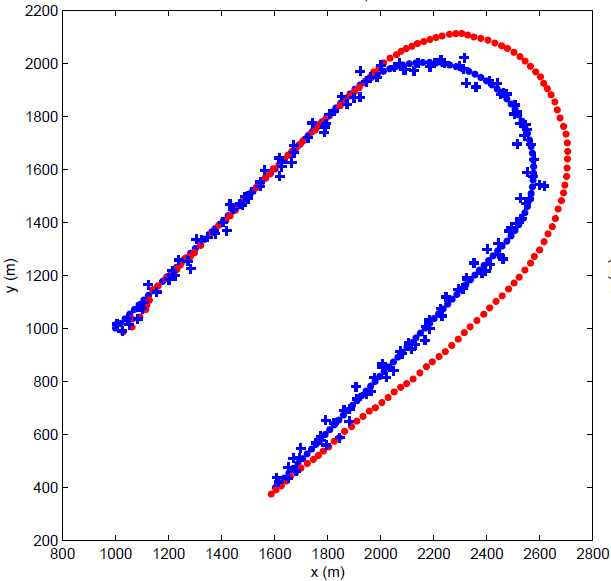
\includegraphics[scale=0.3333]{./img/maneuver}
	\end{figure}
\end{frame}
\begin{frame}
	\frametitle\insertsection
	\framesubtitle\insertsubsection
	\vspace{-2em}
	\begin{block} {Approaches to maneuvering problems}
		\begin{itemize}
			\item {Maneuver Detection}
			\item {Multiple Models}
			\begin{itemize}
				\item {Non-switching mutiple models}
				\item {Switching mutiple models}
				\begin{itemize}
					\item {Generalized Pseudo Bayesian (GPB) methods}
					\item {Interacting Multiple Model (IMM) algorithm}
				\end{itemize}
			\end{itemize}
		\end{itemize}
	\end{block}
\end{frame}
\begin{frame}
	\frametitle\insertsection
	\framesubtitle\insertsubsection
	\vspace{-2em}
	\begin{block} {Multiple Model Approaches}
		\begin{itemize}
			\item {Multiple parallel filters}
			\item {Each filter is based on one of following:}
			\begin{itemize}
				\item {Different Motion model.}
				\item {Different Process noise.}
			\end{itemize}
			\item {Overall estimate is a weighted combination of the estimates from the multiple filters.}
			\item {No explicit maneuver detection.}
		\end{itemize}
	\end{block}
\end{frame}
\begin{frame}
	\frametitle\insertsection
	\framesubtitle\insertsubsection
	\vspace{-2em}
	\begin{block} {Probability Model}
		\begin{itemize}
			\item {For each model, compute the probability to determine which model is correct. }
			\item {The probability that model $j$ is correct is}
			\begin{align*}
				P\{M_j | Z^k\} = \frac{\Lambda_j(k) \mu_j}{\sum\limits_{l=1}^r \Lambda_l(k)\mu_l}
			\end{align*}
			\vspace{-2em}
			\begin{align*}
				\text{with\ }	\Lambda_j(k) = \frac{1}{\sqrt{2\pi|\mathbf{S}_j(k)|}}\exp[-\frac{1}{2}\mathbf{v}^\intercal_j(k)\mathbf{S}_j(k)\mathbf{v}_j(k)]
			\end{align*}
			$\mu_j$ : prior probability (the probability that model $j$ was correct after update).
		\end{itemize}
	\end{block}
\end{frame}
\begin{frame}
	\frametitle\insertsection
	\framesubtitle\insertsubsection
	\vspace{-2em}
	\begin{block}{Interacting Multiple Model (IMM) Filter}
		\begin{itemize}
			\item {A method for combining state hypotheses from multiple filter models}
			\item {The objective is to get a better state estimate of targets with changing dynamics}
			\item {The filter models can be selected to match the behavior of targets of interest.}
			\item {Model management is governed by an underlying Markov chain that controls the switching behavior among the multiple models.}
		\end{itemize}
	\end{block}
\end{frame}
\begin{frame}
	\frametitle\insertsection
	\framesubtitle\insertsubsection
	\vspace{-1em}
	\begin{figure}
		\caption{\textbf{IMM Filter : Functional Diagram}}
		\scalebox{1}{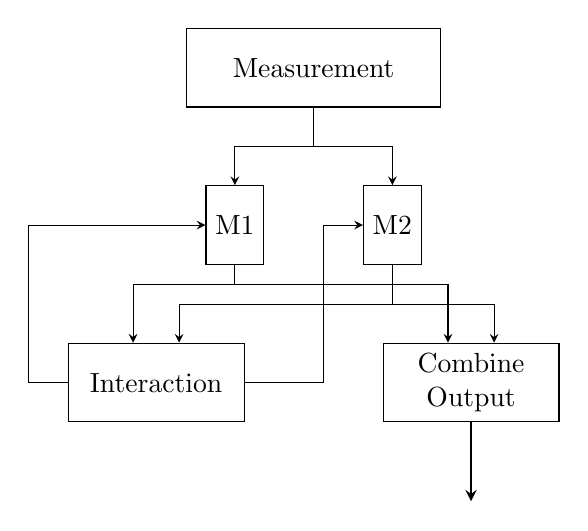
\begin{tikzpicture}[xscale=1,yscale=1,
	square/.style={rectangle, minimum height=10mm, draw=black, align=center},
	round/.style={circle, inner sep=0pt, fill=red!50, opacity=0.75, align=center},
	point/.style={circle, inner sep=0pt, minimum size=2mm, align=center},
	oval/.style={ellipse, fill=gray!50, opacity=0.75},
	label/.style={text width=5mm, align=center},
	node distance= 3cm and 1cm, >=stealth]
	
	%Nodes
	\node[square, text width=30mm]	(measurement)	at (0,0) {Measurement};
	\node[square]	(m1)	at	(-1,-2)	{M1};
	\node[square]	(m2)	at	(1,-2)	{M2};
	\node[square, text width=20mm]	(interact)	at	(-2,-4)	{Interaction};
	\node[square, text width=20mm]	(combine)	at	(2,-4)	{Combine Output};
	
	%Lines
	\draw[black, ->] (measurement.south) -- ++(0,-0.5) -| (m1.north);
	\draw[black, ->] (measurement.south) -- ++(0,-0.5) -| (m2.north);
	\draw[black, ->] (m1.south) -- ++(0,-0.25) -| (interact.120);
	\draw[black, ->] (m1.south) -- ++(0,-0.25) -| (combine.120);
	\draw[black, ->] (m2.south) -- ++(0,-0.5) -| (interact.60);
	\draw[black, ->] (m2.south) -- ++(0,-0.5) -| (combine.60);
	
	\draw[black, ->] (interact.west) -- ++(-0.5,0) |- (m1.west);
	\draw[black, ->] (interact.east) -- ++(1,0) |- (m2.west);
	
	\draw[black, thick, ->] (combine.south) -- ++(0,-1);	
\end{tikzpicture}}
	\end{figure}
\end{frame}
\begin{frame}
	\frametitle\insertsection
	\framesubtitle\insertsubsection
	\vspace{-2em}
	\begin{figure}
		\caption{\textbf{IMM Filter : Algorithms}}
		\scalebox{0.75}{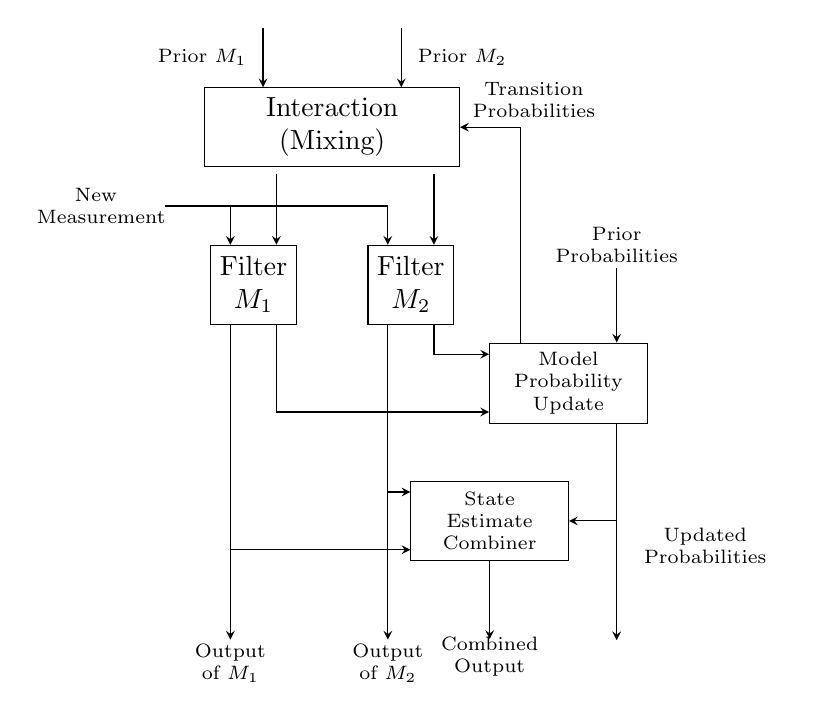
\begin{tikzpicture}[xscale=1,yscale=1,
	square/.style={rectangle, minimum height=10mm, draw=black, align=center},
	round/.style={circle, inner sep=0pt, fill=red!50, opacity=0.75, align=center},
	point/.style={circle, inner sep=0pt, minimum size=2mm, align=center},
	oval/.style={ellipse, fill=gray!50, opacity=0.75},
	label/.style={text width=5mm, align=center, font=\scriptsize},
	node distance= 3cm and 1cm, >=stealth]
	
	%Nodes
	\node[square, text width=30mm]	(interact)	at (0,0) {Interaction\\(Mixing)};
	\node[square]	(m1)	at	(-1,-2)	{Filter\\$M_1$};
	\node[square]	(m2)	at	(1,-2)	{Filter\\$M_2$};
	\node[square, minimum width=20mm, font=\scriptsize]	(prob)	at	(3,-3.25)	{Model\\Probability\\Update};
	\node[square, minimum width=20mm, font=\scriptsize]	(combine)	at	(2,-5)	{State\\Estimate\\Combiner};
	
	
	%Labels
	\node[label, text width=15mm]	(label1)	at (-3,-1)	{New\\Measurement};
	
	%Lines
	\draw[black, <-] (m1.60) -- ++(0,0.9);
	\draw[black, <-] (m2.60) -- ++(0,0.9);
	\draw[black, <-] (interact.30) -- node[label, right, xshift=-10, text width=20mm] {Prior $M_2$} ++(0,0.75);
	\draw[black, <-] (interact.150) -- node[label, left, xshift=10, text width=20mm] {Prior $M_1$} ++(0,0.75);
	\draw[black, ->] (label1.east) -| (m1.120);
	\draw[black, ->] (label1.east) -| (m2.120);
	\draw[black, ->] (m1.300) |- (prob.200);
	\draw[black, ->] (m2.300) |- (prob.160);
	\draw[black, ->] (m1.240) |- (combine.200);
	\draw[black, ->] (m2.240) |- (combine.160);
	\draw[black, ->] (prob.320) |- (combine);
	\draw[black, ->] (prob.140) |- node[label, above, xshift=5, text width=20mm] {Transition\\ Probabilities} (interact.east);
	\draw[black, <-] (prob.40) -- node[label, above, yshift=12, text width=20mm] {Prior\\Probabilities} ++(0,0.95);
	\draw[black, ->] (prob.320) -- node[label, right, yshift=-5, text width=20mm] {Updated Probabilities} ++(0,-2.75);
	
	\draw[black, ->] (m1.240) -- node[label, below, yshift=-55, text width=10mm] {Output of $M_1$} ++(0,-4);
	\draw[black, ->] (m2.240) -- node[label, below, yshift=-55, text width=10mm] {Output of $M_2$} ++(0,-4);
	\draw[black, ->] (combine) -- node[label, below, yshift=-10, text width=20mm] {Combined Output} ++(0,-1.5);
\end{tikzpicture}}
	\end{figure}
\end{frame}
\begin{frame}
	\frametitle\insertsection
	\framesubtitle\insertsubsection
	\vspace{-2em}
	\begin{figure}
		\caption{\textbf{Example : IMM Filter with CV, CA and CT Models}}
		\scalebox{0.8}{\begin{tikzpicture}[xscale=1,yscale=1,
	square/.style={rectangle, minimum height=10mm, draw=black, align=center},
	point/.style={circle, thick, draw=blue, inner sep=0pt, minimum size=1.5mm},
	label/.style={text width=5mm, font=\footnotesize},
	node distance= 1.25cm and 1cm, >=stealth]
	
	%Nodes
	\node[square, minimum width=20mm, minimum height=30mm]	(mixing)	at (0,0)	{Mixing};
	\node[square, xshift=4cm, yshift=2.5mm]	(ca)	[right of=mixing]	{Filter CA};
	\node[square]	(cv)	[above of=ca]		{Filter CV};
	\node[square]	(ct)	[below of=ca]		{Filter CT};
	\node[square, minimum width=30mm, xshift=2.5cm, yshift=-5mm]	(combine)	[below of=ct]		{Combination};
	\node[point]	(sw0)	at (2,1.625)	{};
	\node[point]	(sw1)	at (2,1.875)	{};
	\node[point]	(sw2)	at (2.5,1.75)	{};
	\node[label, blue, text width=20mm]	(dap)	at (3,2.25)	{DAPs enabled};
	
	%Lines
	\draw[black, <-] (mixing.west) -- node[label, below, text width=30mm] {$\hat{\mathbf{X}}^2_{k-1|k-1}\ \mathbf{P}^2_{k-1|k-1}$} ++(-2,0);
	\draw[black, <-] (mixing.135) -- node[label, below, text width=30mm] {$\hat{\mathbf{X}}^1_{k-1|k-1}\ \mathbf{P}^1_{k-1|k-1}$} ++(-2,0);
	\draw[black, <-] (mixing.225) -- node[label, below, text width=30mm] {$\hat{\mathbf{X}}^3_{k-1|k-1}\ \mathbf{P}^3_{k-1|k-1}$} ++(-2,0);
	\draw[black, <-] (mixing.south) -- ++(0,-0.5) -- node[label, below, text width=30mm] {$\mu^{i|j}_{k-1|k-1}$} ++(-3,0);
	
	\draw[black, ->] (mixing.east) -- node[label, below, text width=30mm] {$\hat{\mathbf{X}}^{02}_{k-1|k-1}\ \mathbf{P}^{02}_{k-1|k-1}$} ++(3.38,0);
	\draw[black, ->] (mixing.50) -- node[label, below, text width=30mm] {$\hat{\mathbf{X}}^{01}_{k-1|k-1}\ \mathbf{P}^{01}_{k-1|k-1}$} ++(3.38,0);
	\draw[black, ->] (mixing.310) -- node[label, below, text width=30mm] {$\hat{\mathbf{X}}^{03}_{k-1|k-1}\ \mathbf{P}^{03}_{k-1|k-1}$} ++(3.38,0);
	
	\draw[black, ->] (cv.east) -- ++(5,0) node[label, below, text width=30mm] {$\hat{\mathbf{X}}^1_{k|k}\ \mathbf{P}^1_{k|k}$};
	\draw[black, ->] (ca.east) -- ++(5,0) node[label, below, text width=30mm] {$\hat{\mathbf{X}}^2_{k|k}\ \mathbf{P}^2_{k|k}$};;
	\draw[black, ->] (ct.east) -- ++(5,0) node[label, below, text width=30mm] {$\hat{\mathbf{X}}^3_{k|k}\ \mathbf{P}^3_{k|k}$};;
	
	\draw[black, ->] (combine.east) -- ++(1.85,0) node[label, below, text width=30mm] {$\hat{\mathbf{X}}_{k|k}\ \mathbf{P}_{k|k}$\\$\mu^j_k \ \mu^{i|j}_{k|k}$};
	\draw[black, <-] (combine.150) -- ++(0,3.75) node[label, below, text width=30mm, xshift=0.9cm] {$\hat{\mathbf{X}}^1_{k|k}\ \Lambda^1_k$\\$\mathbf{P}^1_{k|k}$};
	\draw[black, <-] (combine.north) -- node[label, above, text width=30mm, xshift=0.9cm] {$\hat{\mathbf{X}}^2_{k|k}\ \Lambda^2_k$\\$\mathbf{P}^2_{k|k}$} ++(0,2.5);
	\draw[black, <-] (combine.30) -- node[label, above, text width=30mm, xshift=0.9cm, yshift=-5mm] {$\hat{\mathbf{X}}^3_{k|k}\ \Lambda^3_k$\\$\mathbf{P}^3_{k|k}$} ++(0,1.25);
	\draw[black, <-] (combine.west) -- ++(-9.25,0) node[label, below, text width=30mm, xshift=1.5cm] {$\mu^j_{k-1} (i,j = 1,2,3)$};
	
	\draw[blue, thick, ->] (sw2) -- ++(1.875,0);
	\draw[blue, thick, <-] (ca.160) -- ++(-0.5,0) -- ++(0,1.19);
	\draw[blue, thick, <-] (ct.160) -- ++(-0.5,0) -- ++(0,1.25);
	
	\draw[blue, thick, -] (sw1) -- (sw2);
	\draw[blue, thick, <-] (sw0) -- ++(-3,0) node[label, text width=30mm, xshift=-7mm] {$\mathbf{Z}_k=[x_k\ y_k\ z_k]^\intercal$};
	\draw[blue, thick, <-] (sw1) -- ++(-1,0) node[label, above, text width=50mm, xshift=-5mm] {$\mathbf{Z}_k=[x_k\ y_k\ z_k\ \dot{x}_k\ \dot{y}_k\ \dot{z}_k]^\intercal$};
\end{tikzpicture}}
	\end{figure}
\end{frame}
\begin{frame}
	\frametitle\insertsection
	\framesubtitle\insertsubsection
	\vspace{-2em}
	\begin{block}{IMM Design}
		\begin{itemize}
			\item {Model Set Design -- Most important}
			\begin{itemize}
				\item {Most designs are ad-hoc.}
				\item {Need enough models.}
				\item {Models must be different enough so that their performance differences are "identifiable" or "observable".}
			\end{itemize}
			\item {Design of Transition Probability Matrix (TPM)}
			\begin{itemize}
				\item {Done a priori.}
				\item {Algorithms for online adaption are a current research area.}
			\end{itemize}
		\end{itemize}
	\end{block}
\end{frame}
%\subsection{A General State Estimation Framework}
%\begin{frame}
%	\frametitle\insertsection
%	\framesubtitle\empty
%	\begin{center}
%		\Large \textbf{\insertsubsection}
%	\end{center}
%\end{frame}
%\begin{frame}
%	\frametitle\insertsection
%	\framesubtitle\insertsubsection
%	\vspace{-2em}
%	\begin{block}{MATLAB}
%		\begin{itemize}
%			\item {Easy to use}
%			\item {Weak type}
%			\item {Slow processing}
%		\end{itemize}
%	\end{block}
%	\begin{block}{Object Oriented Languages}
%		\begin{itemize}
%			\item {Fast}
%			\item {Object oriented}
%			\item {Can be implemented.}
%		\end{itemize}
%	\end{block}
%\end{frame}
%\begin{frame}
%	\frametitle\insertsection
%	\framesubtitle\insertsubsection
%	\begin{table}
%		\caption{\textbf{Classes and their implementations}}
%		\begin{tabular}{|c|c|c|c|} \hline
%			\rowcolor{aerolightblue}
%			\textbf{Model} & \textbf{Noise} & \textbf{Estimator} & \textbf{IO} \\ \hline
%			LinearModel & Gaussian & Kalman Filter & ASTERIX \\ \hline
%			MultiModel & & Extended Kalman Filter & XML \\ \hline
%			GenericModel & & Unscented Kalman Filter & \\ \hline
%			 & & IMM Filter & \\ \hline
%			 & & Particle Filter & \\ \hline
%		\end{tabular}
%	\end{table}
%\end{frame}